% Early detection of manufacturing-defective cells. Style: no em or en dashes; short captions.
Section~\ref{sec:problem} established that cell-to-cell variability dominates within the G1
group, where nominally identical cells span a thirteenfold range in final SOH. A practical
question follows. Can the defective cells be identified early, before their capacity has visibly
diverged? We find that they can, but only from the shape of the discharge voltage curve, not from
any scalar health indicator.

\subsection{Scalar indicators are blind within a group}\label{sec:screen_scalar}
Within G1, the early-life value and slope of the discharge capacity, the surface-temperature
resistance proxy, the coulombic efficiency, and the DC internal resistance all fail to separate
the fast-failing cells from the robust ones. Every within-group rank correlation with final SOH
is weak and not significant, with $|\rho|<0.32$ and $p>0.2$. In other words, at fixed operating
condition the standard health indicators carry no early warning of which cell will fail.

\subsection{The voltage curve carries an early signature}\label{sec:screen_dqv}
The discriminative signal instead lies in how the discharge capacity voltage curve evolves. We
use the Severson descriptor, the change in the curve between an early reference cycle and a later
screening cycle, $\Delta Q(V)=Q_{j}(V)-Q_{i}(V)$~\cite{severson2019data}, summarised by
$\log_{10}\mathrm{Var}\,\Delta Q(V)$. Evaluated at a screening cycle of 100, this scalar
classifies eventual early death, defined as final SOH below 0.80, at a leave-one-out AUC of 0.78,
well above the 0.64 obtained from the scalar capacity value alone in Section~\ref{sec:problem}.
The same descriptor and cutoff reproduce on the independent MIT LFP corpus, at AUC 0.75 and with a
Pearson correlation of $-0.88$ between $\log_{10}\mathrm{Var}\,\Delta Q(V)$ and log cycle life.
This gives a usable screen by cycle 100 on both a large-format and a small-format LFP dataset.

\subsection{How early is the warning}\label{sec:screen_early}
The distinctive value of the voltage signature is that it appears before the capacity signal.
Figure~\ref{fig:screen} plots the detection AUC against the screening cycle for a classifier built
on the voltage descriptor and for one built on the observed capacity fade trajectory. At cycle 50
the capacity trajectory carries no usable prospective signal: with so few cycles the fitted
fade-slope direction does not generalise across cells and its leave-one-out AUC collapses toward
zero, whereas the SIT voltage descriptor already discriminates at an AUC of 0.65, the only signal
above the scalar capacity ceiling at that point. By cycle 75 the capacity trajectory has caught up,
and by cycle 100 it slightly exceeds the voltage descriptor. The MIT cross-validation follows the
same pattern, becoming reliable only by cycle 100. We therefore make a deliberately bounded claim.
The voltage descriptor buys roughly 50 cycles of lead time over the capacity trajectory on the SIT
cells, identifying which cells will fail before the capacity fade reveals it; once enough cycles
accumulate, the capacity trajectory itself suffices. The descriptor does not by itself sharpen the
prediction of when or how far a given cell will collapse. That regression task remains bounded by
the difficulty documented in Section~\ref{sec:rul_results}.

\begin{figure}[pos=t]
\centering
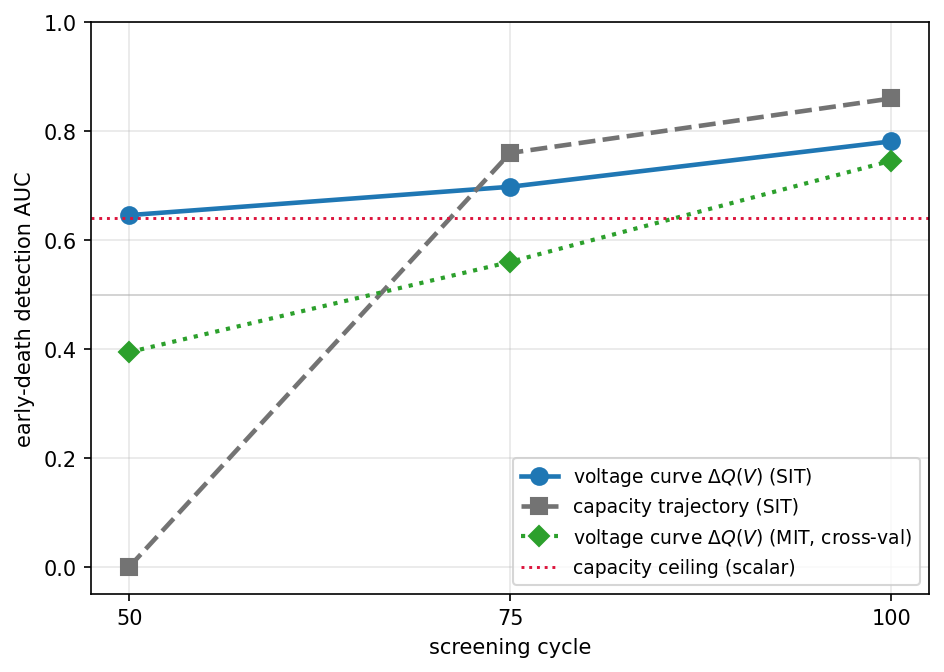
\includegraphics[width=\linewidth]{figures/fig_screening.png}
\caption{Early detection AUC versus screening cycle.}\label{fig:screen}
\end{figure}
